\documentclass[11pt,a4paper]{article}
\usepackage[T1]{fontenc}
\usepackage{lmodern,amsmath,amssymb,graphicx,booktabs,longtable,array,float,tikz}
\usepackage[margin=25mm]{geometry}
\usepackage[hidelinks]{hyperref}
\usepackage{fancyhdr}
\pagestyle{fancy}\fancyhf{}\lhead{Lamb-Wave Simulation in Aluminum Plates}\rhead{Group 11}\cfoot{\thepage}
\setlength{\headheight}{14pt}\setlength{\parindent}{0pt}\setlength{\parskip}{6pt}
\begin{document}\hypersetup{pageanchor=false}
\begin{titlepage}\centering\vspace*{25mm}
{\LARGE\bfseries Simulation of Lamb-Wave Propagation in an Aluminum Plate for Defect Detection\par}
\vspace{18mm}{\large Instructor: Dr. Ganjiani\par}\vspace{12mm}{\large Group 11\par}\vspace{6mm}
\begin{tabular}{ll}Pouya Asghari&810600037\\Mehdi Gharibshahi&810601248\\Arash Bakhtiari&810601192\end{tabular}
\vfill{\large Winter 1404 (Iranian calendar)\par}
\end{titlepage}\hypersetup{pageanchor=true}
\section*{About this English edition}
This edition translates the supplied Persian group report, preserving its procedure, figures, interpretations, and conclusions. Original Abaqus screenshots are retained. Figure~\ref{fig:1} is redrawn with English labels using the stated dimensions; its original raster is also supplied. The small-hole radius is not specified in the source text and has not been invented. A separate editorial appendix identifies reproduction limits and qualifications. Simulations were not rerun during conversion. Three original simulation videos accompany the repository; native Abaqus models, input decks, scripts, and raw sensor histories were not present in the supplied archive.
\section*{Abstract}
This report investigates the propagation of elastic Lamb waves in aluminum plates for detecting defects and holes. Owing to their ability to travel long distances and their sensitivity to thickness changes and structural discontinuities, Lamb waves are useful tools for nondestructive testing (NDT) and structural health monitoring (SHM). The main objective is to compare wave behavior and received signals for an intact plate and a plate containing a hole, using the finite element method (FEM) in Abaqus. For the defined geometry, changes in waveform, amplitude reduction, and scattering caused by wave interaction with the hole are evaluated.
\clearpage\tableofcontents\newpage\listoffigures\newpage
\section{Introduction}
Continuous structural health monitoring in aerospace, automotive, and mechanical engineering is important for preventing sudden failures. Aluminum plates are widely used in these industries because of their high strength-to-weight ratio. Lamb waves are elastic waves that propagate in thin solid plates; particle motion includes components normal to the plate and along the direction of propagation. Their principal advantage is their ability to cover large areas with relatively little energy loss.

When these waves encounter discontinuities such as cracks, thickness reductions, or holes, physical phenomena including reflection, scattering, and mode conversion occur. By receiving and analyzing the resulting signal changes, the presence and potentially the location of a defect can be inferred.
\section{Theory and fundamentals of Lamb-wave propagation}
Lamb waves generally propagate in two main groups: symmetric modes ($S_0,S_1,\ldots$) and antisymmetric modes ($A_0,A_1,\ldots$). A characteristic feature is dispersion: propagation speed depends on plate thickness and excitation frequency.

In defect-detection problems, the plate is often excited by a concentrated force acting as a high-frequency pulse, for example a Hanning-windowed pulse. In a uniform medium, wave energy spreads through the plate in a regular pattern. A hole introduces a new free boundary, producing reflected and scattered waves that change the signal's time of flight and distort the received amplitude. The specific pulse used in this project is described in Section~\ref{sec:pulse}; the general Hanning-pulse example does not establish that such a window was used here.
\section{Problem definition and model geometry}
According to the problem statement, two aluminum-plate models, each measuring $100\times100$ mm with a thickness of 1 mm, are considered to compare the influence of a hole on wave propagation:
\begin{itemize}
\item \textbf{Model 1: intact plate.} A continuous, defect-free plate serves as the reference.
\item \textbf{Model 2: perforated plate.} A plate of the same dimensions contains a circular hole of radius 25 mm. Its center lies 30 mm from the bottom edge and 30 mm from the right edge.
\end{itemize}
\begin{figure}[H]\centering
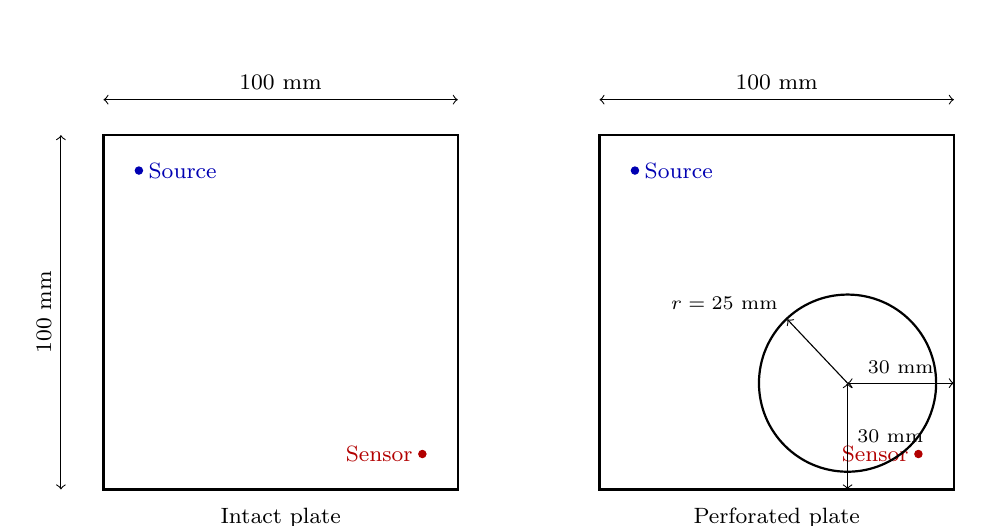
\begin{tikzpicture}[x=0.45cm,y=0.45cm,font=\footnotesize]
\foreach \dx/\lab in {0/Intact plate,14/Perforated plate}{
\begin{scope}[shift={(\dx,0)}]
\draw[thick] (0,0) rectangle (10,10);
\draw[<->] (0,11)--node[above]{100 mm}(10,11);
\fill[blue!70!black] (1,9) circle (0.12) node[right]{Source};
\fill[red!70!black] (9,1) circle (0.12) node[left]{Sensor};
\node at (5,-0.8){\lab};
\end{scope}}
\draw[<->] (-1.2,0)--node[left,rotate=90,anchor=south]{100 mm}(-1.2,10);
\draw[thick] (21,3) circle (2.5);
\draw[->] (21,3)--(19.3,4.8) node[above left]{\scriptsize $r=25$ mm};
\draw[dashed] (21,3)--(24,3);
\draw[<->] (21,3)--node[above]{\scriptsize 30 mm}(24,3);
\draw[<->] (21,0)--node[right]{\scriptsize 30 mm}(21,3);
\end{tikzpicture}
\caption{Schematic of the two primary configurations, redrawn with English labels from the source dimensions. Source and sensor are 10 mm from their adjacent edges.}\label{fig:1}\end{figure}

\subsection{Boundary conditions and loading}
For both models, the plate edges are fully constrained, with all translational displacement degrees of freedom fixed:
\begin{equation}U_1=U_2=U_3=0.\end{equation}
Excitation is applied as a concentrated force at a point 10 mm from the top and left edges. The receiver is located 10 mm from the bottom and right edges, where the displacement history is recorded.
\section{Finite element simulation in Abaqus}
This section describes material definition, meshing, the dynamic explicit step, boundary conditions, amplitude-based loading, and history-output extraction.
\subsection{Geometry and material definition}
A square plate is first created in the software.
\begin{figure}[H]\centering
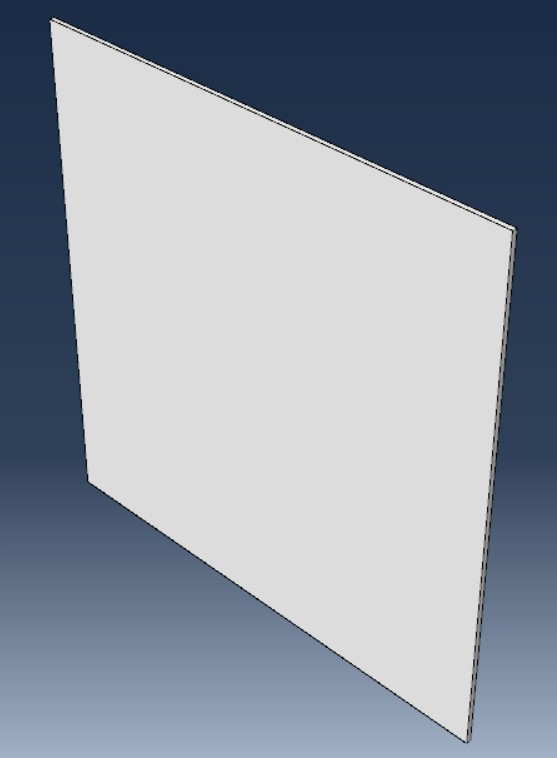
\includegraphics[width=.85\linewidth,height=.38\textheight,keepaspectratio]{figures/rId13.jpeg}
\caption{Square plate.}\label{fig:2}\end{figure}

The plate is then partitioned to create four intersection nodes, two of which coincide with the actuator and receiver locations.
\begin{figure}[H]\centering

\includegraphics[width=.85\linewidth,height=.38\textheight,keepaspectratio]{figures/rId14.jpeg}
\caption{Partitioning the plate.}\label{fig:3}\end{figure}

The material of the plate is then defined.
\begin{figure}[H]\centering
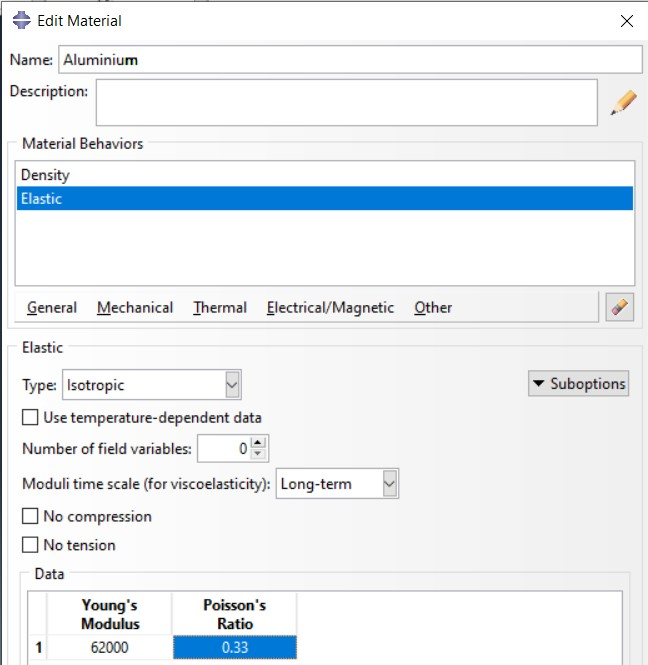
\includegraphics[width=.47\linewidth,height=.40\textheight,keepaspectratio]{figures/rId15.jpeg}\hfill
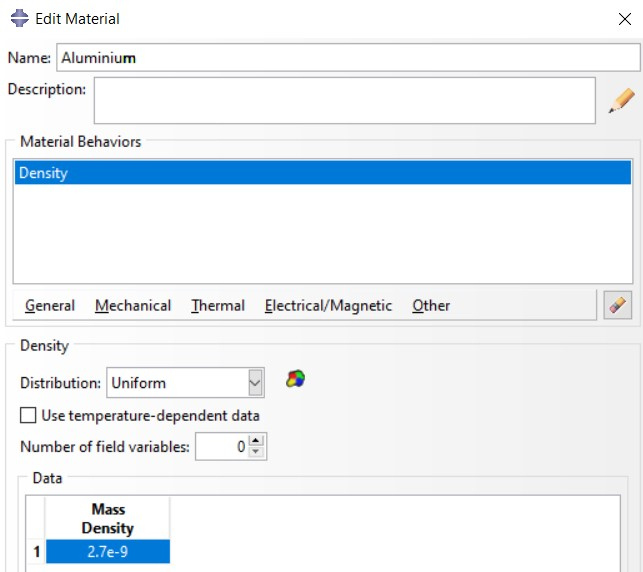
\includegraphics[width=.47\linewidth,height=.40\textheight,keepaspectratio]{figures/rId16.jpeg}
\caption{Mechanical properties and density of the aluminum plate.}\label{fig:4}\end{figure}

The source screenshots show Young's modulus 62000, Poisson's ratio 0.33, and density $2.7\times10^{-9}$. These numerical entries are retained without silently assigning units; the likely consistent unit interpretation is discussed in the editorial appendix.
\subsection{Dynamic explicit analysis step}
A \texttt{Dynamic, Explicit} step is defined with a duration of 0.1 ms. This short duration is chosen because wave propagation is rapid, and a very small time increment is necessary to resolve the simulation. The screenshot gives a step time of $10^{-4}$ and a maximum time increment of $10^{-7}$.
\begin{figure}[H]\centering
\begin{minipage}[c]{.40\linewidth}\centering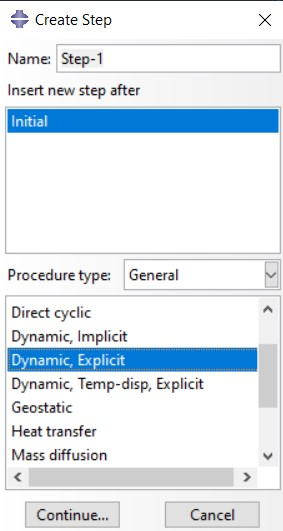
\includegraphics[width=\linewidth,height=.34\textheight,keepaspectratio]{figures/rId19.jpeg}\end{minipage}\hfill
\begin{minipage}[c]{.55\linewidth}\centering
\includegraphics[width=\linewidth]{figures/rId20.jpeg}\par\vspace{6mm}
\includegraphics[width=\linewidth]{figures/rId21.jpeg}\end{minipage}
\caption{Create Step dialog and time settings.}\label{fig:5}\end{figure}

\subsection{Boundary conditions and measurement points}
The project statement requires the perimeter of the aluminum plate to be fixed. A displacement boundary condition is used, and the side faces are selected and constrained.
\begin{figure}[H]\centering
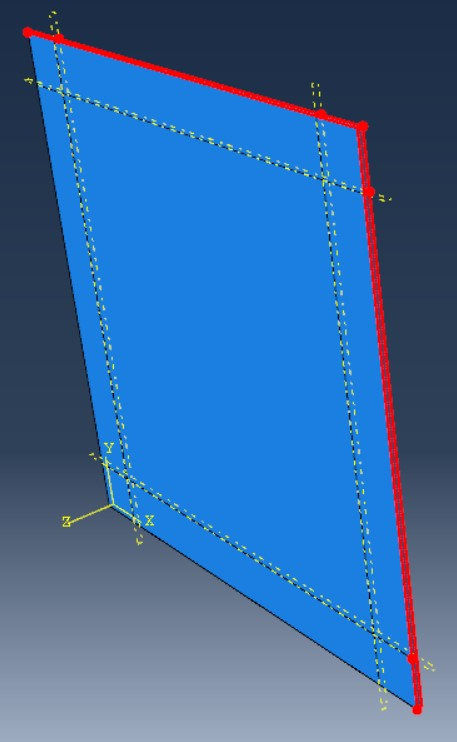
\includegraphics[width=.47\linewidth,height=.40\textheight,keepaspectratio]{figures/rId25.jpeg}\hfill
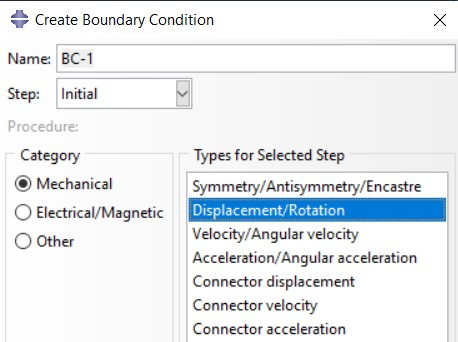
\includegraphics[width=.47\linewidth,height=.40\textheight,keepaspectratio]{figures/rId26.jpeg}
\caption{Defining the boundary condition.}\label{fig:6}\end{figure}

The $U_1$, $U_2$, and $U_3$ options are selected to fix the plate.
\begin{figure}[H]\centering
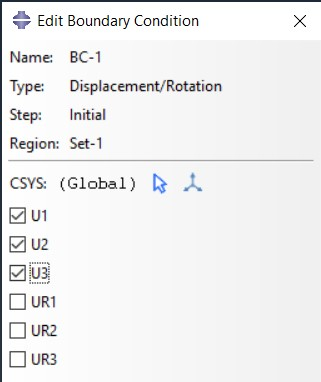
\includegraphics[width=.85\linewidth,height=.38\textheight,keepaspectratio]{figures/rId29.jpeg}
\caption{Edit Boundary Condition dialog.}\label{fig:7}\end{figure}

The constraints can then be seen on the model. Two point sets are also created at the actuator and sensor nodes.
\begin{figure}[H]\centering
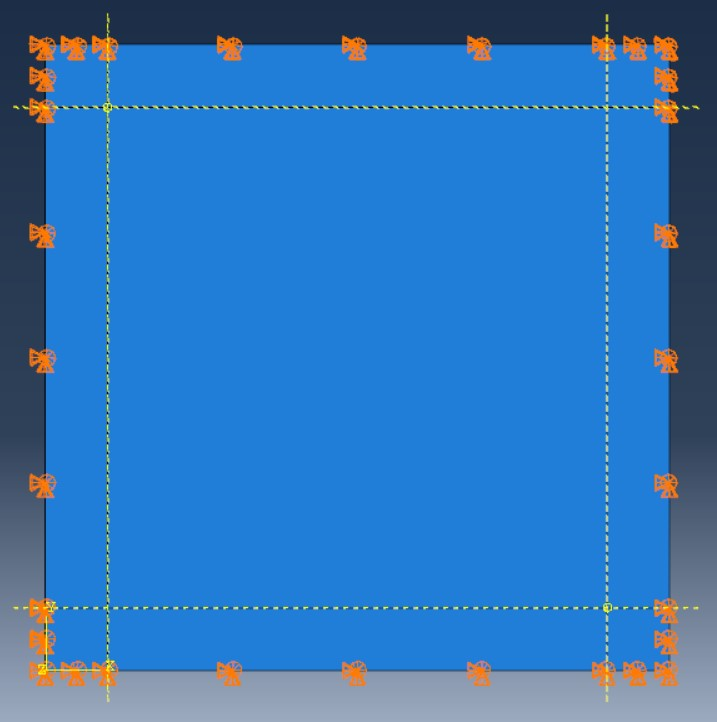
\includegraphics[width=.85\linewidth,height=.38\textheight,keepaspectratio]{figures/rId30.jpeg}
\caption{Constrained plate with actuator and sensor locations.}\label{fig:8}\end{figure}

\subsection{Concentrated-force excitation}\label{sec:pulse}
The force is applied at the point 10 mm from the top and left edges. As specified by the project, it is a concentrated force.
\begin{figure}[H]\centering
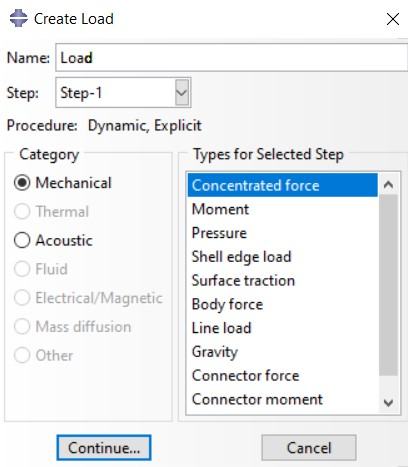
\includegraphics[width=.85\linewidth,height=.38\textheight,keepaspectratio]{figures/rId31.jpeg}
\caption{Create Load dialog.}\label{fig:9}\end{figure}

The force has only an out-of-plane component: $CF_3=1$, while the remaining components are zero.
\begin{figure}[H]\centering
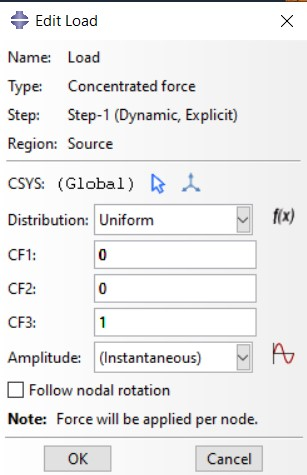
\includegraphics[width=.85\linewidth,height=.38\textheight,keepaspectratio]{figures/rId32.jpeg}
\caption{Edit Load dialog.}\label{fig:10}\end{figure}

A sinusoid-like time variation is entered manually using a tabular amplitude named \texttt{Pulse}, because it acts as a short pulse.
\begin{figure}[H]\centering
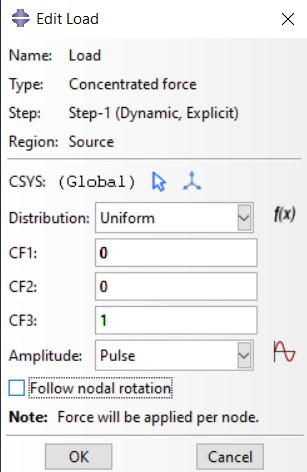
\includegraphics[width=.47\linewidth,height=.40\textheight,keepaspectratio]{figures/rId33.jpeg}\hfill
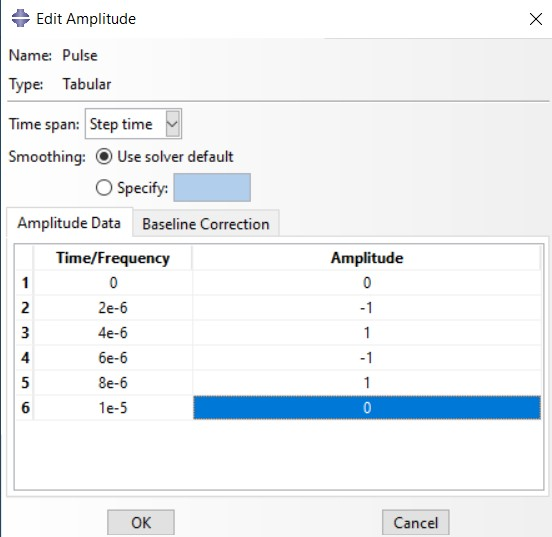
\includegraphics[width=.47\linewidth,height=.40\textheight,keepaspectratio]{figures/rId34.jpeg}
\caption{Edit Amplitude settings for the pulse.}\label{fig:11}\end{figure}

For clarity, the amplitude values visible in the source screenshot are transcribed below. They define a tabular waveform, not an independently verified analytic sine or Hanning function.
\begin{center}\begin{tabular}{rr}\toprule Time (s)&Amplitude multiplier\\\midrule
0&0\\$2\times10^{-6}$&$-1$\\$4\times10^{-6}$&1\\$6\times10^{-6}$&$-1$\\$8\times10^{-6}$&1\\$10^{-5}$&0\\\bottomrule\end{tabular}\end{center}
\subsection{Output requests}
The displacement in the out-of-plane $z$ direction is requested for viewing the results. Field output uses \texttt{Evenly spaced time intervals}, with 100 intervals. History output uses \texttt{Every n time increments}, with $n=1$.
\begin{figure}[H]\centering
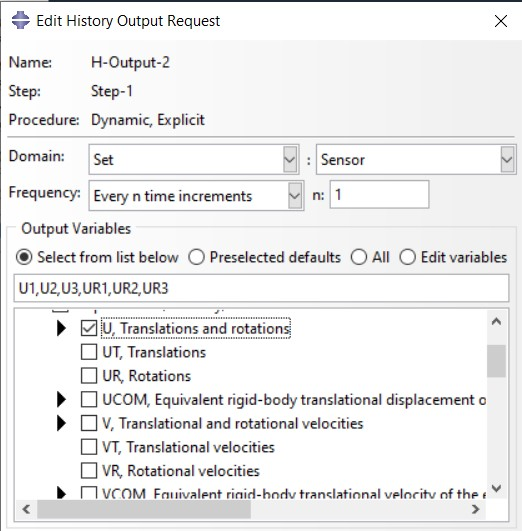
\includegraphics[width=.47\linewidth,height=.40\textheight,keepaspectratio]{figures/rId37.jpeg}\hfill
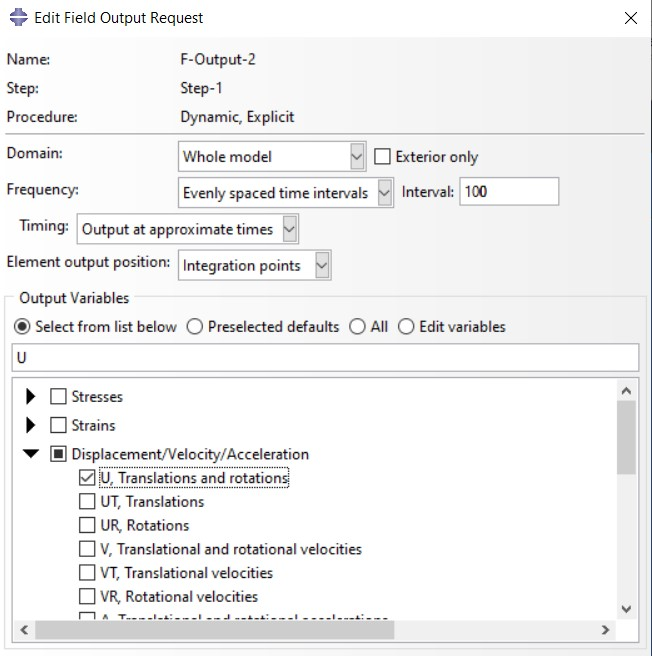
\includegraphics[width=.47\linewidth,height=.40\textheight,keepaspectratio]{figures/rId38.jpeg}
\caption{History and field output settings.}\label{fig:12}\end{figure}

\subsection{Mesh and analysis job}
The plate is then meshed. The Global Seeds screenshot shows an approximate global size of 1 in model length units.
\begin{figure}[H]\centering
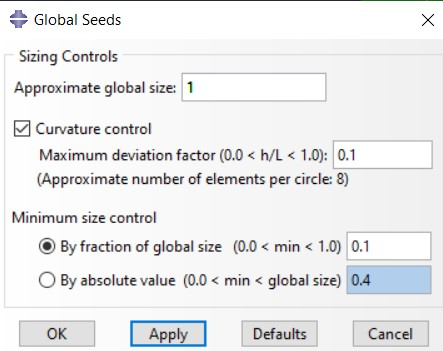
\includegraphics[width=.85\linewidth,height=.38\textheight,keepaspectratio]{figures/rId41.jpeg}
\caption{Global Seeds dialog.}\label{fig:13}\end{figure}
\begin{figure}[H]\centering
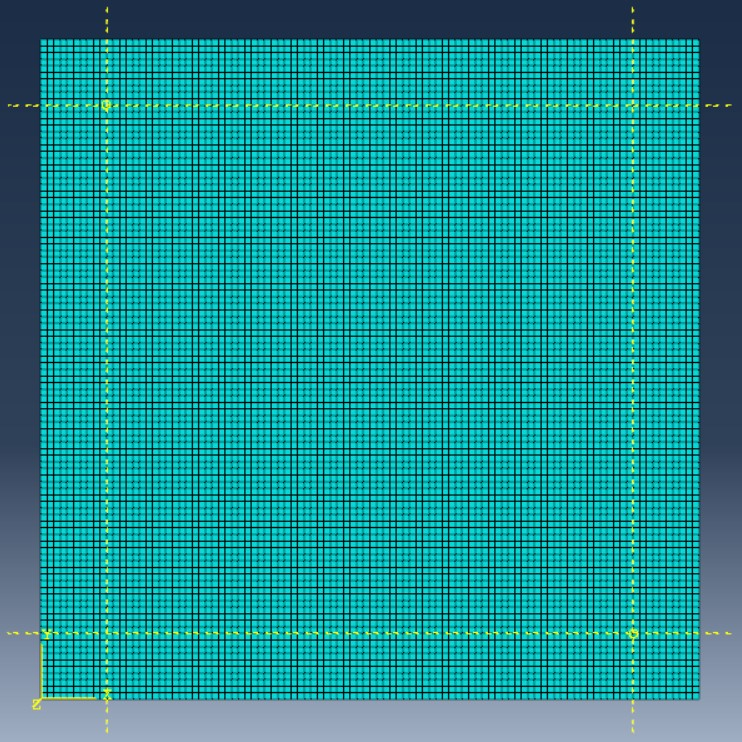
\includegraphics[width=.85\linewidth,height=.38\textheight,keepaspectratio]{figures/rId42.jpeg}
\caption{Meshed intact plate.}\label{fig:14}\end{figure}

Three-dimensional elements are used. The screenshot identifies the Explicit library and the 3D Stress family; it does not establish an exact element designation.
\begin{figure}[H]\centering
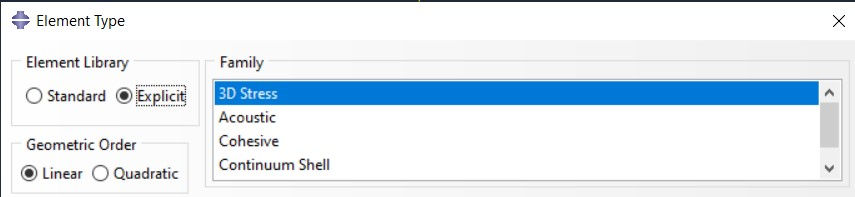
\includegraphics[width=.85\linewidth,height=.38\textheight,keepaspectratio]{figures/rId43.jpeg}
\caption{Element Type dialog.}\label{fig:15}\end{figure}

An analysis job is created. Under Precision, \texttt{Double -- analysis only} is selected.
\begin{figure}[H]\centering
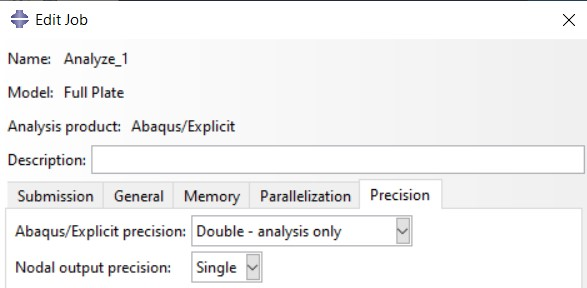
\includegraphics[width=.85\linewidth,height=.38\textheight,keepaspectratio]{figures/rId44.jpeg}
\caption{Edit Job precision settings.}\label{fig:16}\end{figure}

\subsection{Visualization and animation}
The settings shown below are used to make the waves easier to see.
\begin{figure}[H]\centering
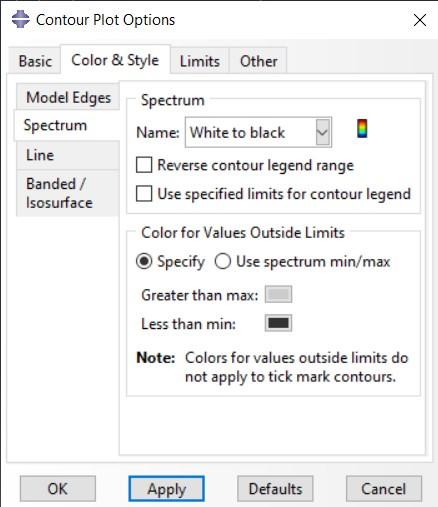
\includegraphics[width=.47\linewidth,height=.40\textheight,keepaspectratio]{figures/rId45.jpeg}\hfill
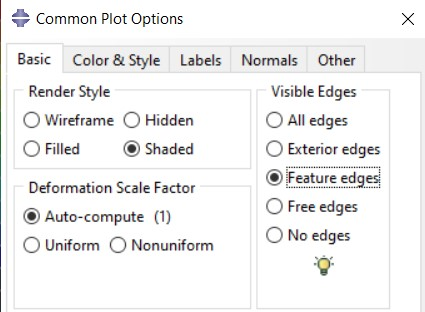
\includegraphics[width=.47\linewidth,height=.40\textheight,keepaspectratio]{figures/rId46.jpeg}
\caption{Visualization settings.}\label{fig:17}\end{figure}

The following figure shows waves in the intact plate.
\begin{figure}[H]\centering
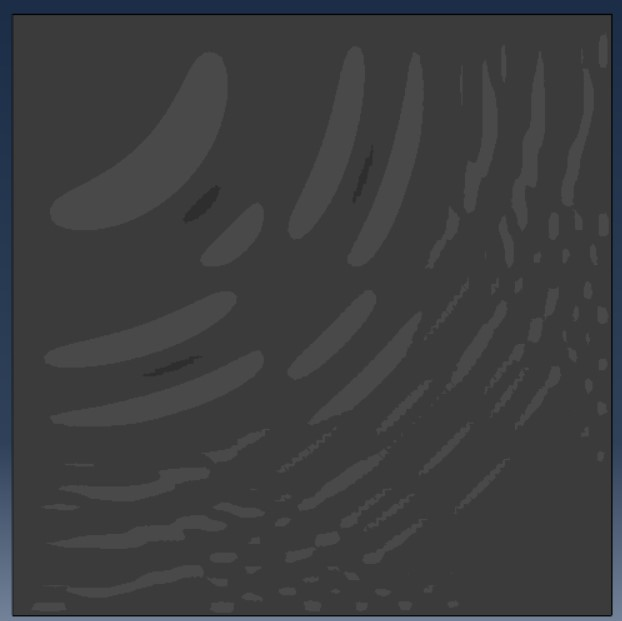
\includegraphics[width=.85\linewidth,height=.38\textheight,keepaspectratio]{figures/rId49.jpeg}
\caption{Waves in the intact plate.}\label{fig:18}\end{figure}

The animation is exported using the settings below. Its video is supplied alongside the report.
\begin{figure}[H]\centering
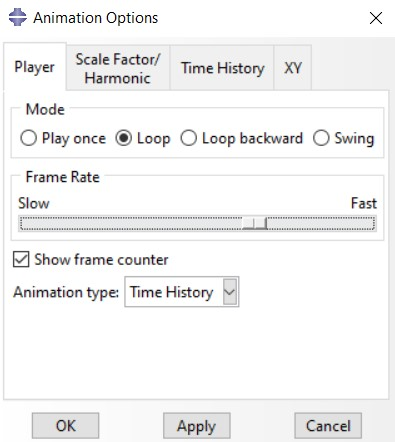
\includegraphics[width=.85\linewidth,height=.38\textheight,keepaspectratio]{figures/rId50.jpeg}
\caption{Animation Options dialog.}\label{fig:19}\end{figure}

\subsection{Plate with a 25 mm radius hole}
For the perforated configuration, the original model is copied, the geometry and mesh are modified to include the 25 mm radius hole, and the new job is submitted.
\begin{figure}[H]\centering
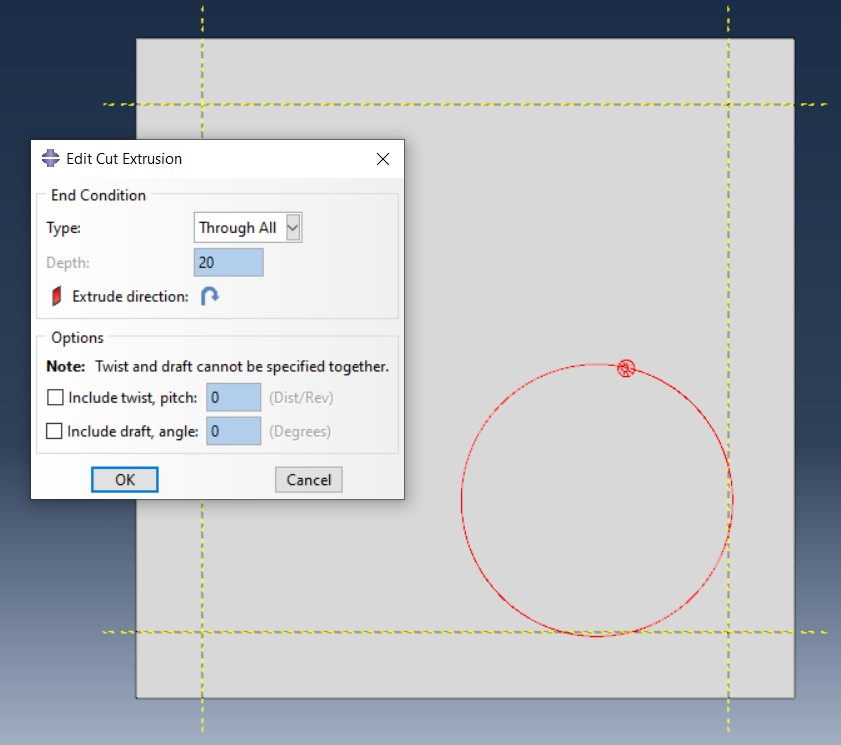
\includegraphics[width=.85\linewidth,height=.38\textheight,keepaspectratio]{figures/rId51.jpeg}
\caption{Creating a circular hole of radius 25 mm.}\label{fig:20}\end{figure}
\begin{figure}[H]\centering
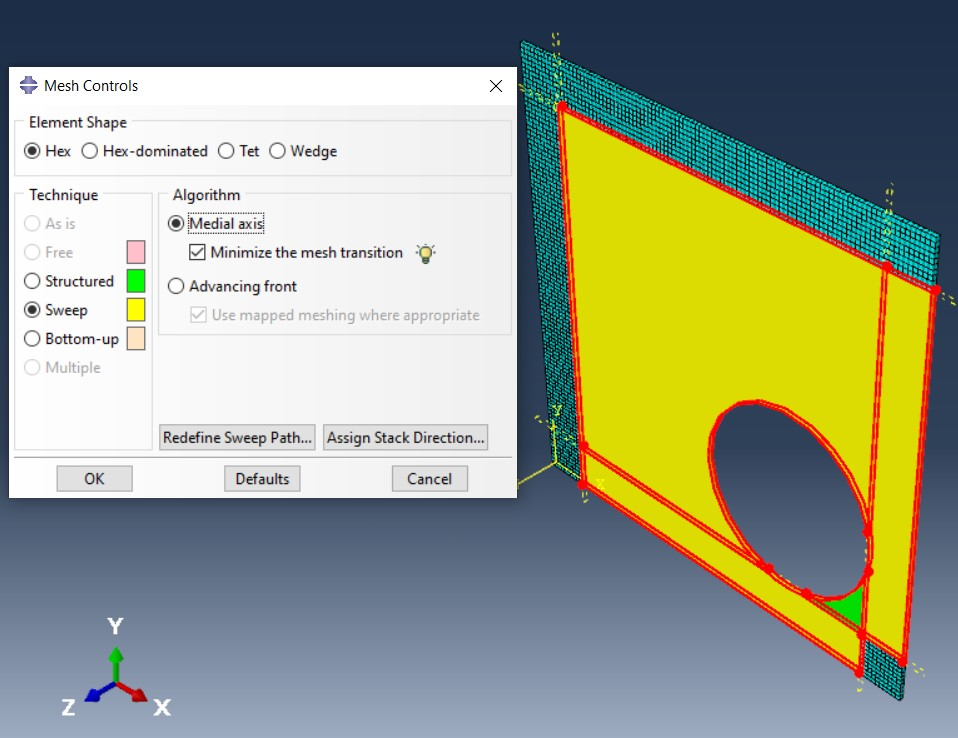
\includegraphics[width=.85\linewidth,height=.38\textheight,keepaspectratio]{figures/rId52.jpeg}
\caption{Mesh Controls for the perforated plate.}\label{fig:21}\end{figure}
\begin{figure}[H]\centering
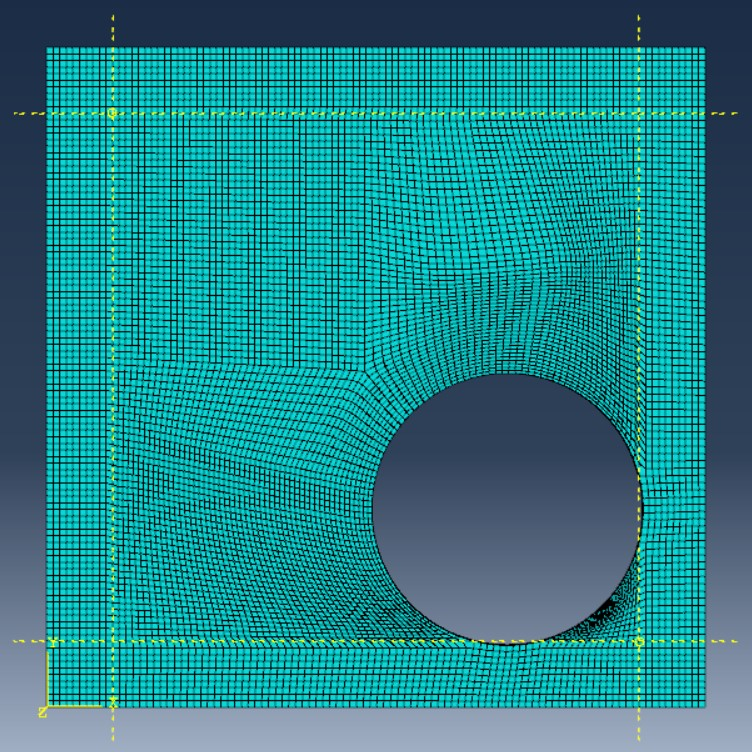
\includegraphics[width=.85\linewidth,height=.38\textheight,keepaspectratio]{figures/rId53.jpeg}
\caption{Meshed perforated plate.}\label{fig:22}\end{figure}
\begin{figure}[H]\centering
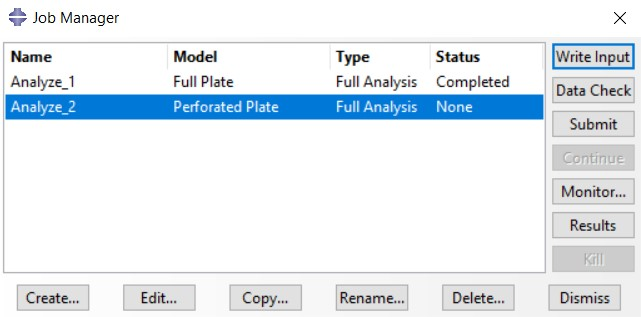
\includegraphics[width=.85\linewidth,height=.38\textheight,keepaspectratio]{figures/rId54.jpeg}
\caption{Job Manager for the intact and perforated cases.}\label{fig:23}\end{figure}

The two simulations are then displayed side by side.
\begin{figure}[H]\centering
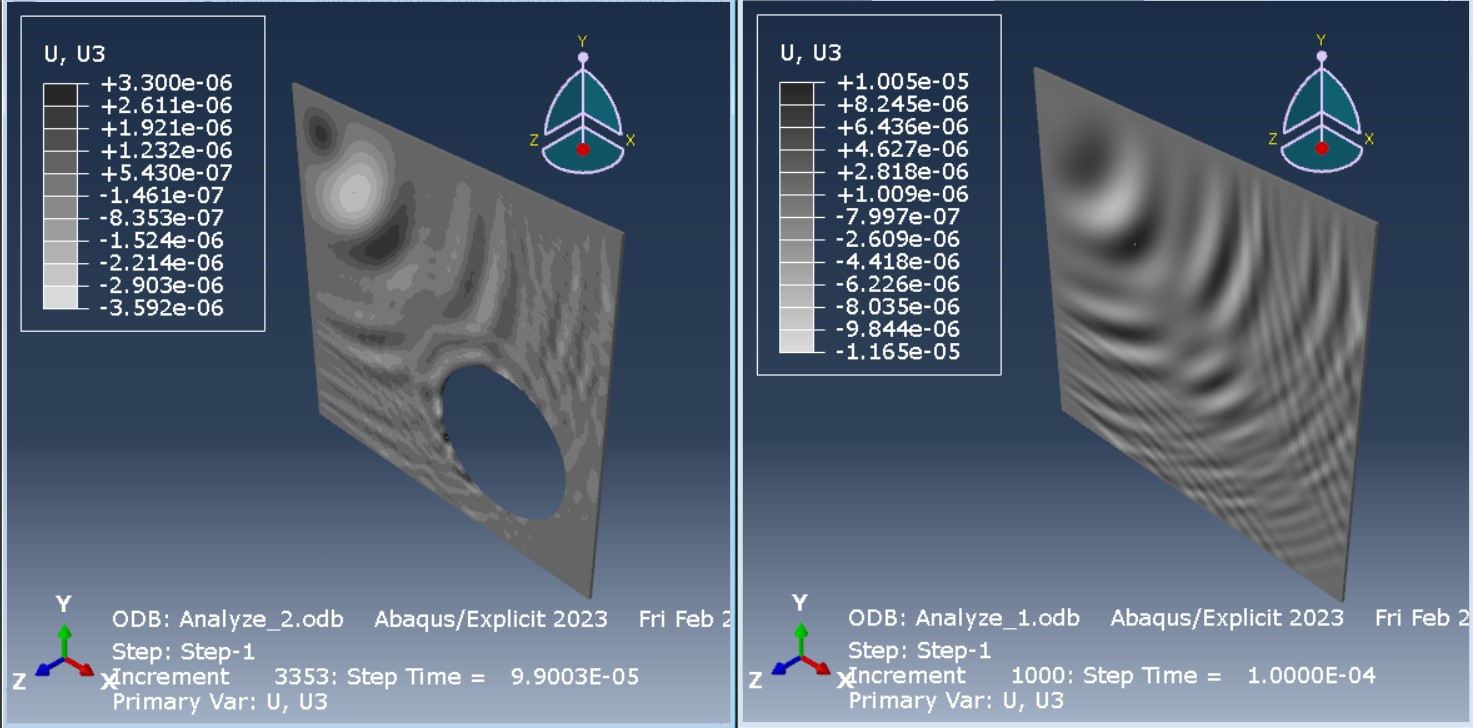
\includegraphics[width=.85\linewidth,height=.38\textheight,keepaspectratio]{figures/rId55.jpeg}
\caption{Side-by-side simulations of the intact and large-hole plates.}\label{fig:24}\end{figure}

The wave pattern is visibly disturbed in the perforated plate. To compare both cases quantitatively in a plot, their out-of-plane displacement components are extracted and drawn on the same axes.
\begin{figure}[H]\centering
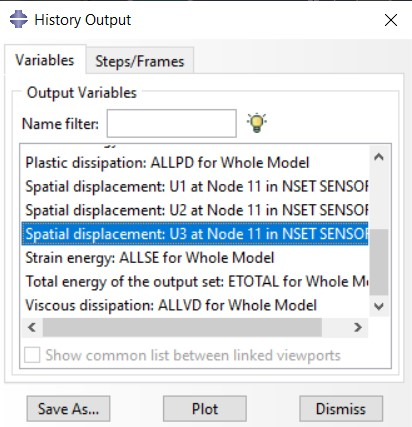
\includegraphics[width=.47\linewidth,height=.40\textheight,keepaspectratio]{figures/rId56.jpeg}\hfill
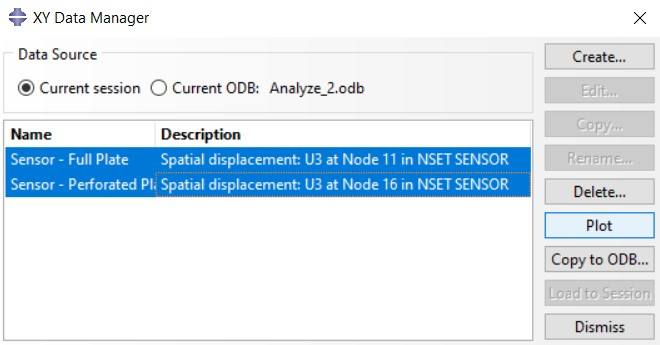
\includegraphics[width=.47\linewidth,height=.40\textheight,keepaspectratio]{figures/rId57.jpeg}
\caption{Extracting displacement histories for both cases.}\label{fig:25}\end{figure}

The resulting histories are shown below.
\begin{figure}[H]\centering
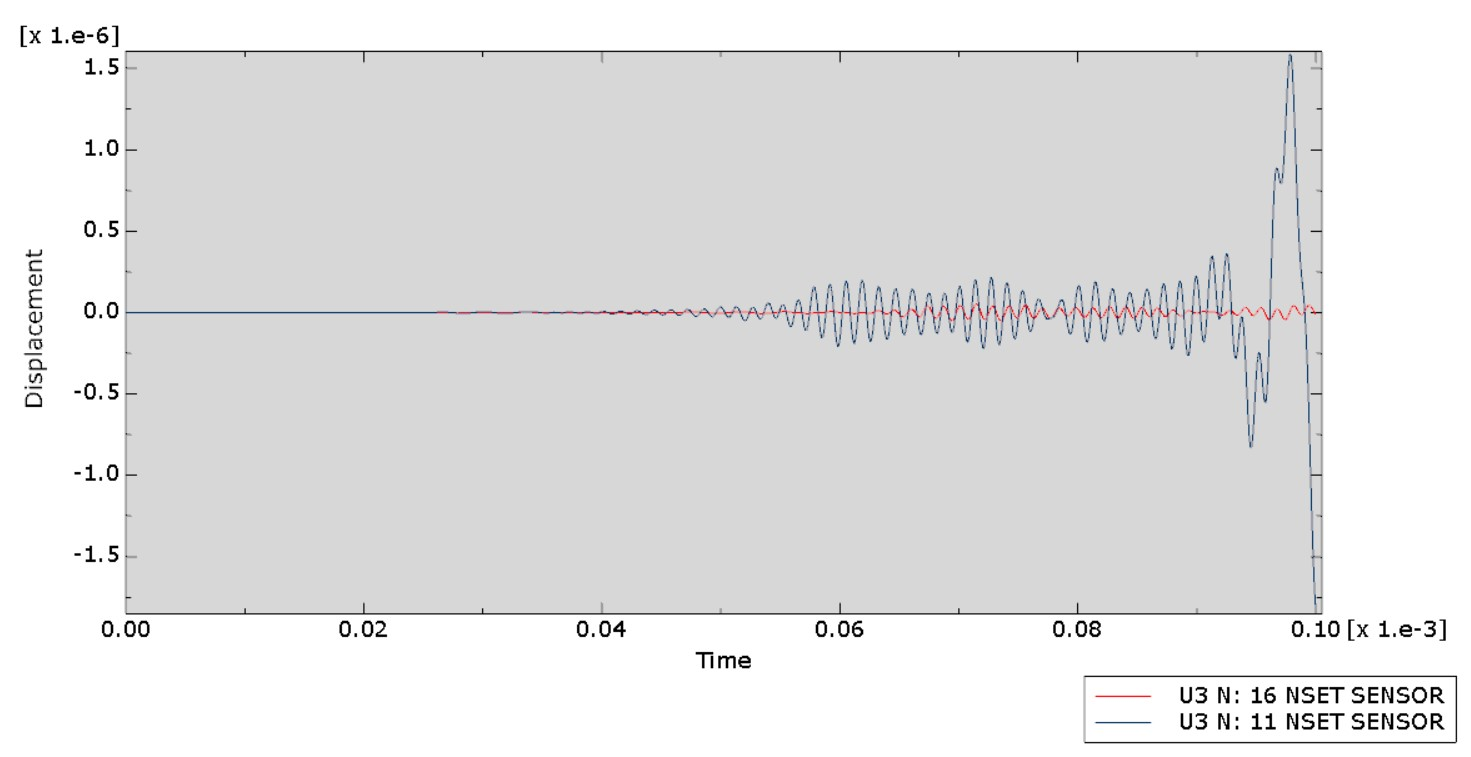
\includegraphics[width=.85\linewidth,height=.38\textheight,keepaspectratio]{figures/rId60.jpeg}
\caption{Displacement histories: intact plate and plate with a 25 mm radius hole.}\label{fig:26}\end{figure}

\section{Interpretation of the large-hole comparison}
The source interprets the plot using elastic Lamb-wave propagation and interaction with discontinuities. It shows out-of-plane displacement $U_3$ as a function of time at the sensor node. The explanations in this section are translated source interpretations, not new independently verified findings.
\subsection{Red curve: intact plate}
\textbf{Cylindrical spreading and amplitude reduction.} In the intact plate, waves generated at the source spread without obstruction in all directions. As the wave moves away from the source, its energy is distributed over a larger wavefront through geometric spreading. Consequently, the displacement amplitude at the opposite sensor is small.

\textbf{Regular pattern.} The source describes the red curve as a smooth, stable dynamic response with an amplitude of approximately $10^{-7}$ m. It interprets this as the direct arrival of undistorted wave packets followed by regular reflections from the outer plate edges. This dimensional amplitude statement is retained from the original prose; the model's length unit must be confirmed before using it quantitatively.
\subsection{Blue curve: plate containing a hole}
The source attributes the strong variations, large oscillations, and spikes to the hole, and offers the following explanations.

\textbf{Constructive interference near a free boundary.} For the defined geometry, the sensor lies near the edge of the large hole. The hole introduces a free boundary along the propagation path. Reflected waves combine with incident waves near this boundary, which the source interprets as constructive interference and strong amplification of $U_3$ in that region.

\textbf{Local stiffness reduction.} Removing a substantial volume of aluminum reduces the local bending stiffness. The source argues that the elastic-wave energy therefore produces larger deformations, or stronger local vibration, around the hole than in the intact plate.

\textbf{Scattering and path changes.} The hole obstructs the direct line of sight between the transmitter and receiver. Waves must travel around it; the source describes these as creeping waves. This changes the wave pattern and delays signal arrival. The strong blue-curve oscillations are interpreted as scattered waves reaching the sensor with different phases.

\textbf{Resonance and energy accumulation.} The very large peak near $0.09\times10^{-3}$ to $0.10\times10^{-3}$ s is attributed by the source to the combined arrival of waves reflected from the outer plate edges and the hole boundary, creating a strong amplified response.
\subsection{Source interpretation summary}
The source concludes that the large changes in amplitude and waveform are the basis of Lamb-wave NDT: the hole transforms a smooth, low-amplitude signal into a strongly oscillating, scattered response with local amplification.
\section{Smaller central hole}
A further configuration contains a smaller hole at the center of the plate. Its radius is smaller than in the previous case, but no numerical radius is stated in the source text. This case is used to illustrate how a smaller hole can still alter received waves.
\begin{figure}[H]\centering
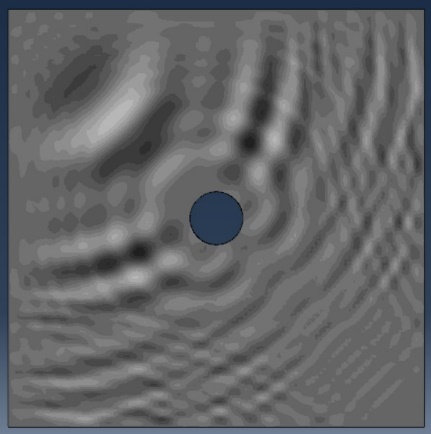
\includegraphics[width=.315\linewidth,height=.34\textheight,keepaspectratio]{figures/rId61.jpeg}\hfill
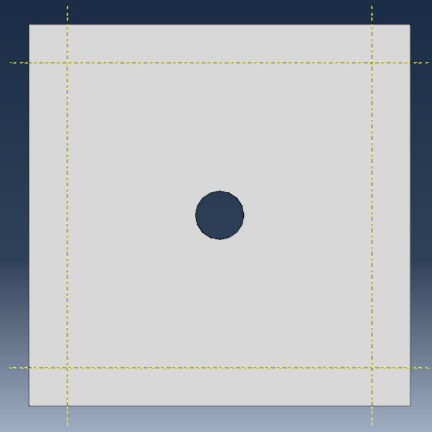
\includegraphics[width=.315\linewidth,height=.34\textheight,keepaspectratio]{figures/rId62.jpeg}\hfill
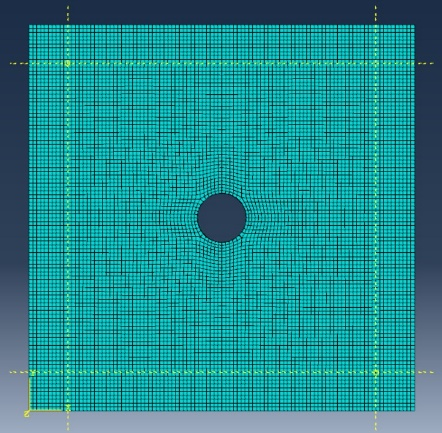
\includegraphics[width=.315\linewidth,height=.34\textheight,keepaspectratio]{figures/rId63.jpeg}
\caption{Geometry, mesh, and simulation for the smaller central hole.}\label{fig:27}\end{figure}

The intact-plate history and the smaller-hole history are plotted together for comparison.
\begin{figure}[H]\centering
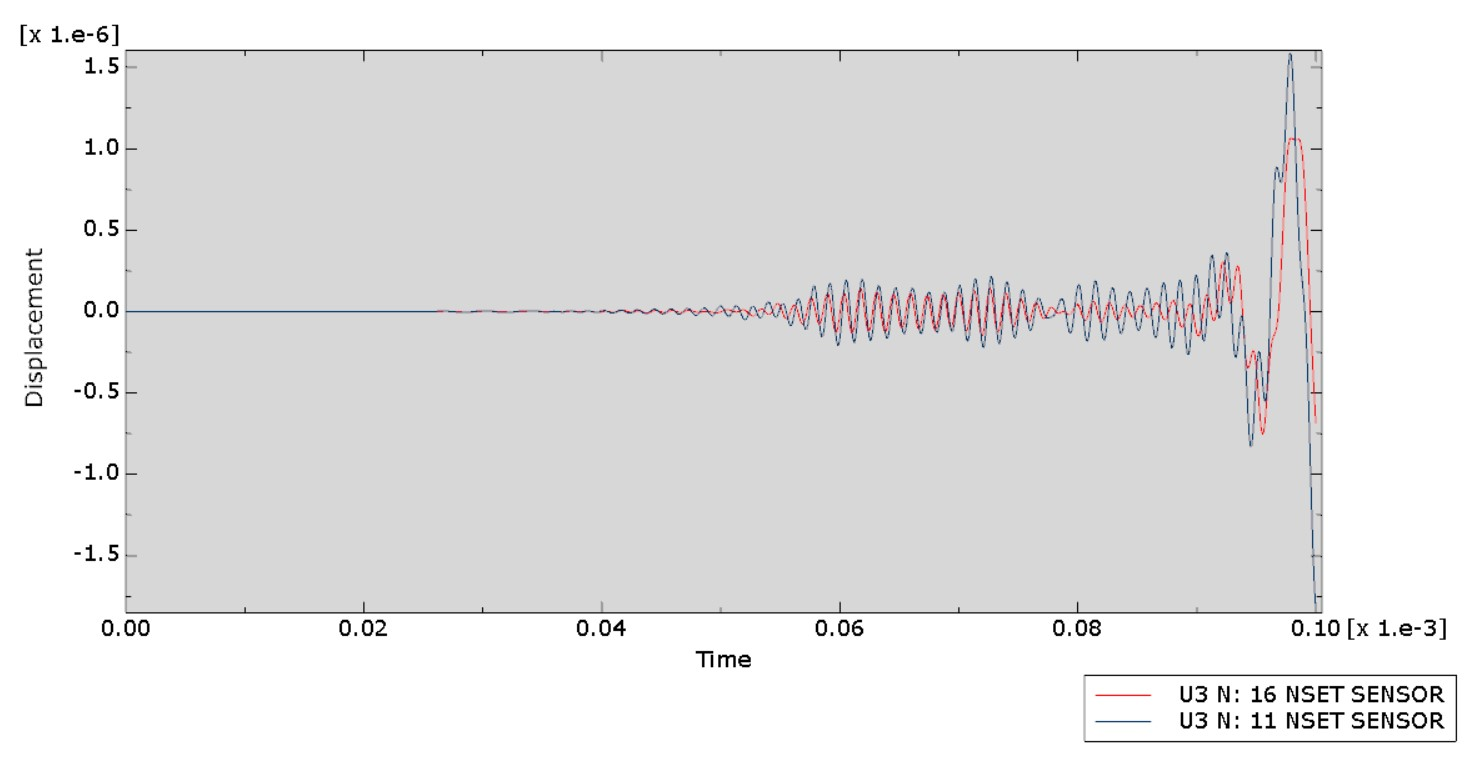
\includegraphics[width=.85\linewidth,height=.38\textheight,keepaspectratio]{figures/rId67.jpeg}
\caption{Intact plate (red) and plate with a smaller central hole (blue).}\label{fig:28}\end{figure}

The source states that the red and blue curves coincide at the beginning of the received response, up to approximately 0.055 ms, because the initial wave travels at the same speed and reaches the sensor. It attributes the subsequent differences and strong blue-curve oscillations to scattering at the hole.

The central hole acts as an obstacle and a free boundary, reflecting and scattering waves in different directions. These waves follow longer paths and arrive later. Their interference with the original wave and with outer-edge reflections produces phase differences and the larger displacement peaks at the end of the blue curve.
\begin{figure}[H]\centering
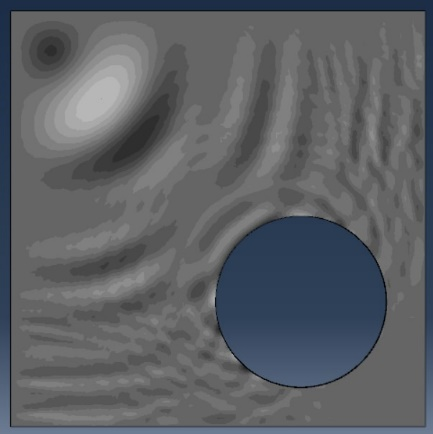
\includegraphics[width=.315\linewidth,height=.34\textheight,keepaspectratio]{figures/rId68.jpeg}\hfill
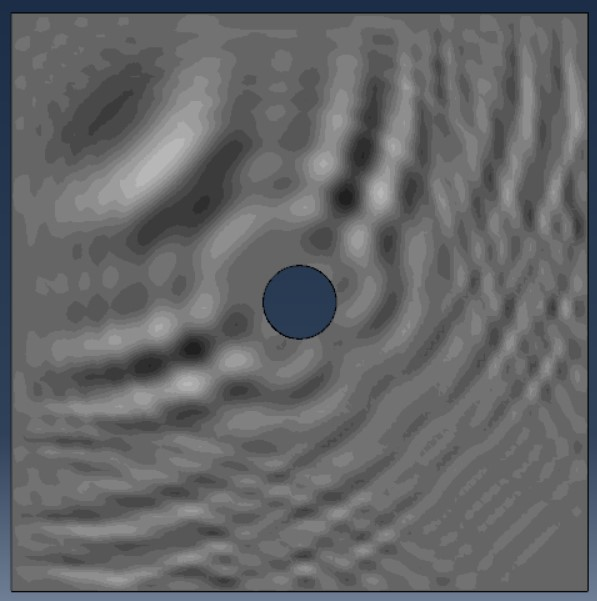
\includegraphics[width=.315\linewidth,height=.34\textheight,keepaspectratio]{figures/rId69.jpeg}\hfill
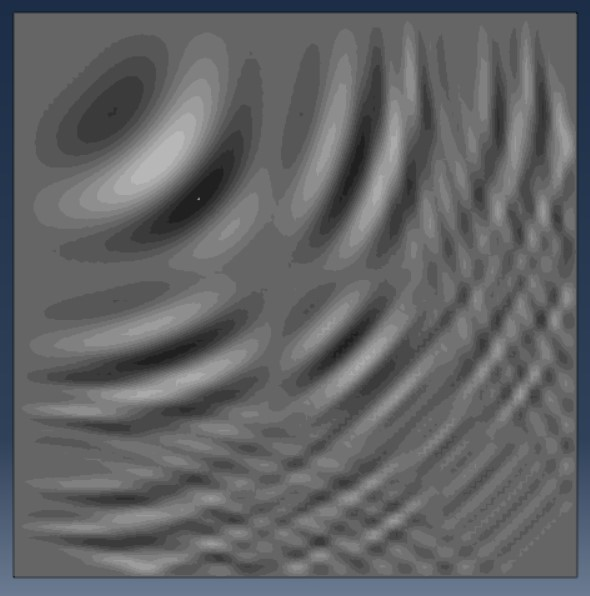
\includegraphics[width=.315\linewidth,height=.34\textheight,keepaspectratio]{figures/rId70.jpeg}
\caption{Wave patterns for all three plate configurations.}\label{fig:29}\end{figure}

\section{Results and discussion}
Extracted sensor displacement--time plots show differences in wave-propagation dynamics. In the intact plate, the incident wave reaches the receiver after following the direct path, followed by regular reflections from the constrained boundaries.

In the perforated model, the 25 mm radius hole obstructs or disturbs the direct path. Energy scatters at the hole boundary. The source describes a reduction in initial signal amplitude and additional wave packets associated with waves scattered around the hole. It states that overlaying the two histories demonstrates the influence of defect geometry on phase delay and elastic-wave energy reduction.

The source also describes amplified late-time peaks in the preceding sections. Both descriptions are preserved here; amplitude changes and transmitted energy require consistent time windows and quantitative measures before these explanations can be reconciled.
\section{Conclusion}
The source concludes that Lamb waves are effective for identifying discontinuities and holes in plate structures. A hole changes received signals through scattering and reflection. Changes in signal amplitude and arrival time are proposed as indicators of a defect. Finite element simulation before physical testing can help interpret wave behavior and guide transmitter and receiver placement.

These are the report's qualitative conclusions. This edition does not add a calibrated detection threshold, a localization algorithm, a sensor-placement optimization, or experimental validation.
\clearpage
\begin{thebibliography}{9}
\bibitem{rose} J. L. Rose, \emph{Ultrasonic Waves in Solid Media}. Cambridge University Press, 1999.\newline\textit{Editorial correction: the Persian source lists 2014. The publisher's front matter gives first publication as 1999.}
\bibitem{su} Z. Su and L. Ye, \emph{Identification of Damage Using Lamb Waves: From Fundamentals to Applications}. Springer Science \& Business Media, 2009.
\bibitem{raghavan} A. Raghavan and C. E. S. Cesnik, ``Review of guided-wave structural health monitoring,'' \emph{The Shock and Vibration Digest}, vol. 39, no. 2, pp. 91--114, 2007.
\bibitem{moser} F. Moser, L. J. Jacobs, and J. Qu, ``Modeling elastic wave propagation in waveguides with the finite element method,'' \emph{NDT \& E International}, vol. 32, no. 4, pp. 225--234, 1999.
\bibitem{alleyne} D. N. Alleyne and P. Cawley, ``The interaction of Lamb waves with defects,'' \emph{IEEE Transactions on Ultrasonics, Ferroelectrics, and Frequency Control}, vol. 39, no. 3, pp. 381--397, 1992.
\bibitem{abaqus} Dassault Syst\`emes SIMULIA Corp., \emph{Abaqus Analysis User's Guide}, Providence, RI, USA, 2023.\newline\textit{Source references are retained for attribution; the referenced works were not all supplied or reviewed during translation.}
\end{thebibliography}
\appendix\clearpage
\section{Editorial notes and reproduction limits}
These notes were added during translation and repository preparation.
\begin{enumerate}
\item \textbf{Available evidence.} The archive contains a Word report and three MP4 videos. It does not include CAE models, INP decks, ODB databases, scripts, or raw XY tables. Native simulations were not opened or rerun. Video frames identify Abaqus/CAE and Abaqus/Explicit 2023.
\item \textbf{Units.} Abaqus inputs require a consistent unit system. The screenshot values $E=62000$, $\rho=2.7\times10^{-9}$, geometry in mm, and step times in seconds are consistent with an N--mm--s--tonne interpretation, giving $E=62000$ MPa and $\rho=2700$ kg/m$^3$. This is an inference from the shown entries, not a unit declaration supplied by a native model. Under that interpretation displacement plots are in mm, so the source's stated $10^{-7}$ m amplitude is not established by the displayed graph alone.
\item \textbf{Pulse and resolution.} The visible tabular pulse is retained. It should not be called a verified Hanning-windowed excitation. Its spectrum, wavelength-to-element-size ratio, through-thickness resolution, exact element formulation, and temporal accuracy need checking. A maximum increment of $10^{-7}$ s does not by itself establish accuracy or convergence.
\item \textbf{Boundary reflections and interpretation.} Fixed edges create reflections. Late-time amplitude growth can include interference and reflected arrivals. The supplied histories alone do not isolate a particular Lamb mode, prove resonance, establish creeping-wave propagation, or determine a reliable defect-detection threshold. Mode identification and dispersion calculations are not supplied.
\item \textbf{Missing parameters.} The small-hole radius, exact element code, through-thickness element count, complete mesh controls, and full input/output definitions cannot be recovered reliably from the report alone. Do not infer the missing radius from screenshot scale.
\item \textbf{Comparison limits.} The source discusses both attenuation and late-time amplification. Raw histories and consistent comparison windows are needed to quantify either effect. No numerical detection accuracy, measured energy loss, convergence study, or experimental validation is supplied.
\item \textbf{Team attribution.} The source is a Group 11 report by Pouya Asghari, Mehdi Gharibshahi, and Arash Bakhtiari. Individual task allocation is not specified. Romanized names should be checked against each contributor's preferred spelling before publication.
\item \textbf{Bibliography.} Reference [1] combines the title of Rose's 1999 book with a 2014 year in the source. The year has been explicitly corrected using the publisher's front matter: \url{https://assets.cambridge.org/97805215/48892/frontmatter/9780521548892_frontmatter.pdf}. Other entries are transcribed from the supplied bibliography rather than claimed as independently verified.
\end{enumerate}
\end{document}
